\documentclass[a4paper,11pt]{article}
\usepackage[utf8]{inputenc}
\usepackage[T1]{fontenc}
\usepackage[slovene]{babel}
\usepackage{graphicx}
\usepackage{url}

\title{Pregled obstoječih rešitev -- Zrno \& Mir d.o.o.}
\author{Leon Kavnik, Naj Rejavc in Ožbi Fric}
\date{24. november 2026}

\begin{document}
\maketitle

\section{Uvod}
Poslovna ideja Zrno \& Mir d.o.o. združuje praženje specialty kave, prodajo kavnih zrn in obratovanje manjše kavarne. Poudarek je na kakovosti, preverjenem poreklu, trajnosti, lokalni skupnosti in prijetni uporabniški izkušnji. Kava bo namenjena posameznikom in podjetjem.

Predlagana spletna rešitev bo obiskovalcem omogočala pregled ponudbe, spoznavanje porekla kave in nakup za domačo uporabo. Rešuje problem nepregledne izbire kav ter pomanjkanja razumljivih informacij za kupce, ki specialty kave še ne poznajo. V nadaljevanju primerjamo tri obstoječe slovenske spletne rešitve.
\newpage
\section{Escobar}
Escobar je pražarna in spletna trgovina z mešanicami, kavami s poreklom, specialty in aromatiziranimi kavami \cite{escobar}.
\textbf{Ključne funkcionalnosti:} katalog kav, prikaz cen in arom oziroma okusov, dodajanje izdelkov v košarico ter predstavitev ponudbe po kategorijah.

\textbf{Prednosti:} široka izbira, pregledne informacije o okusih in poudarek na svežini ter sledljivosti. Kupec lahko izbira glede na svoje želje.

\textbf{Slabosti (lastna ocena):} obsežna ponudba lahko začetniku oteži odločitev; strokovni izrazi o okusih bi lahko zahtevali dodatno razlago.
\begin{figure}[h!]
\centering
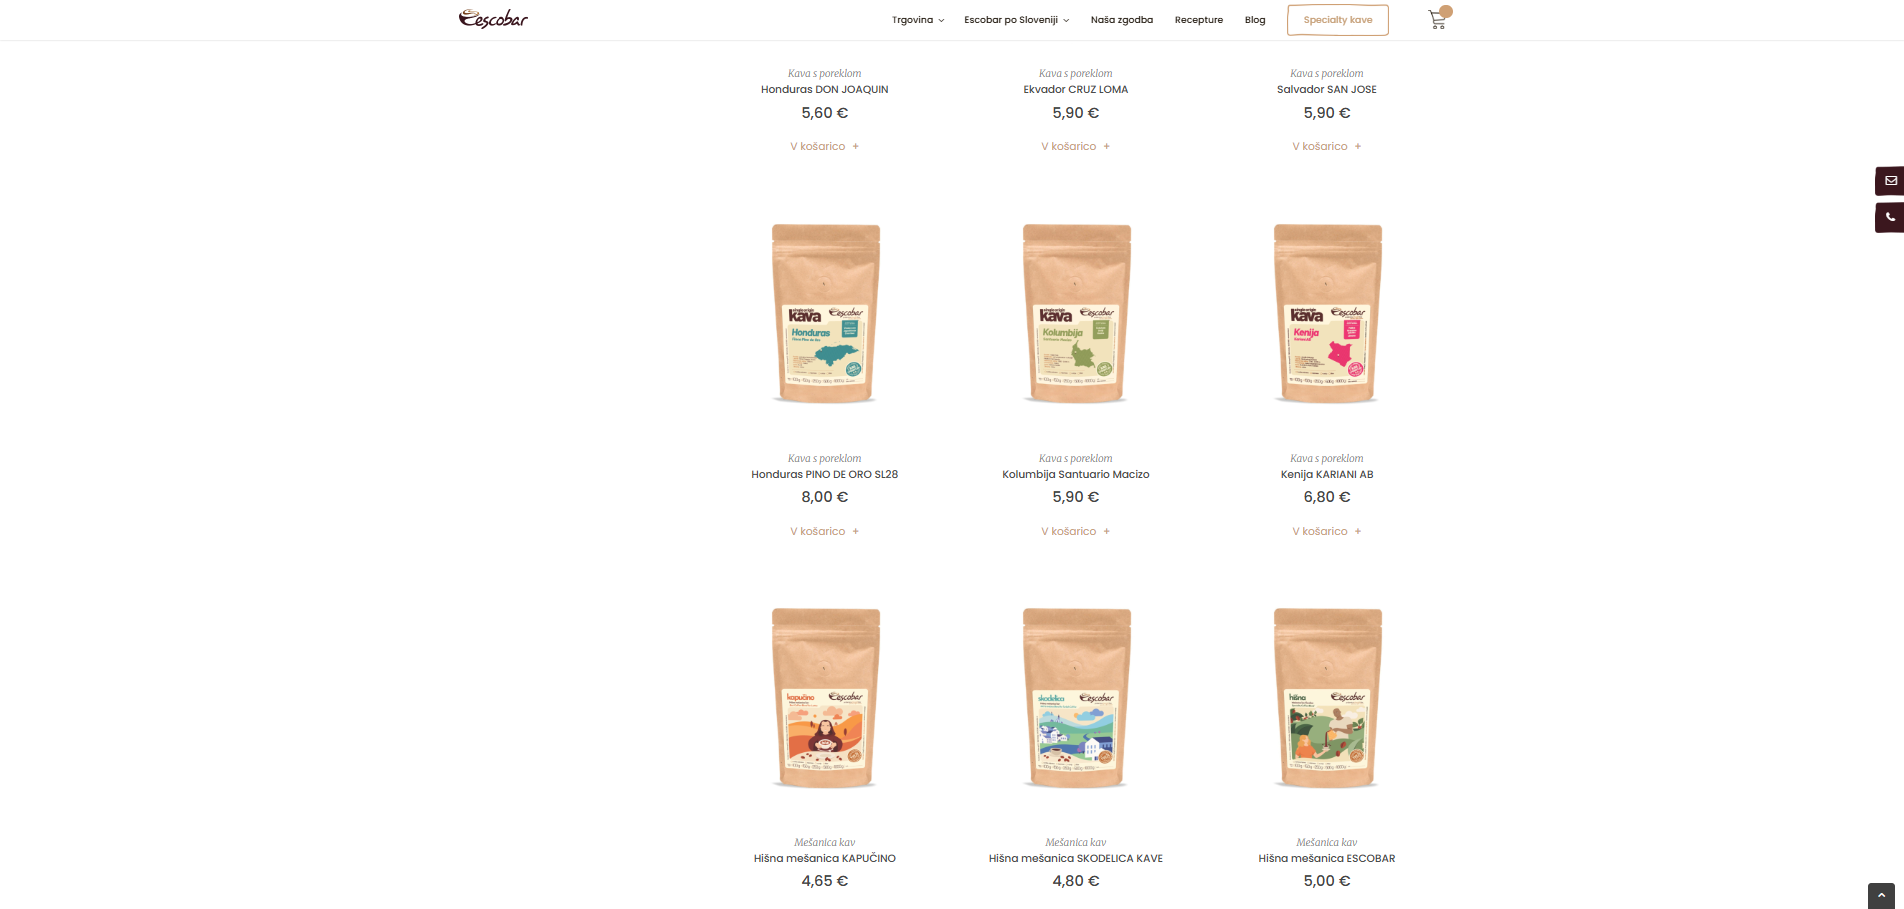
\includegraphics[width=1.0\textwidth]{slike/escobar.png}
\caption{Posnetek zaslona kataloga Escobar \cite{escobar}.}
\end{figure}
\newpage
\section{Pražarna}
Pražarna ponuja specialty kavo, spletno trgovino, izobraževanje o kavi ter poslovno ponudbo za podjetja \cite{prazarna}.

\textbf{Ključne funkcionalnosti:} spletna trgovina, filtriranje po ceni, državi porekla in oceni kakovosti ter ponudba za podjetja.

\textbf{Prednosti:} združevanje prodaje in izobraževanja, strokovna predstavitev priprave kave ter ponudba za poslovne uporabnike.

\textbf{Slabosti (lastna ocena):} številne strokovne vsebine lahko odvrnejo obiskovalca, ki želi zgolj hitro izbrati kavo; za začetnike bi koristila krajša pot do priporočila izdelka.
\begin{figure}[h!]
\centering
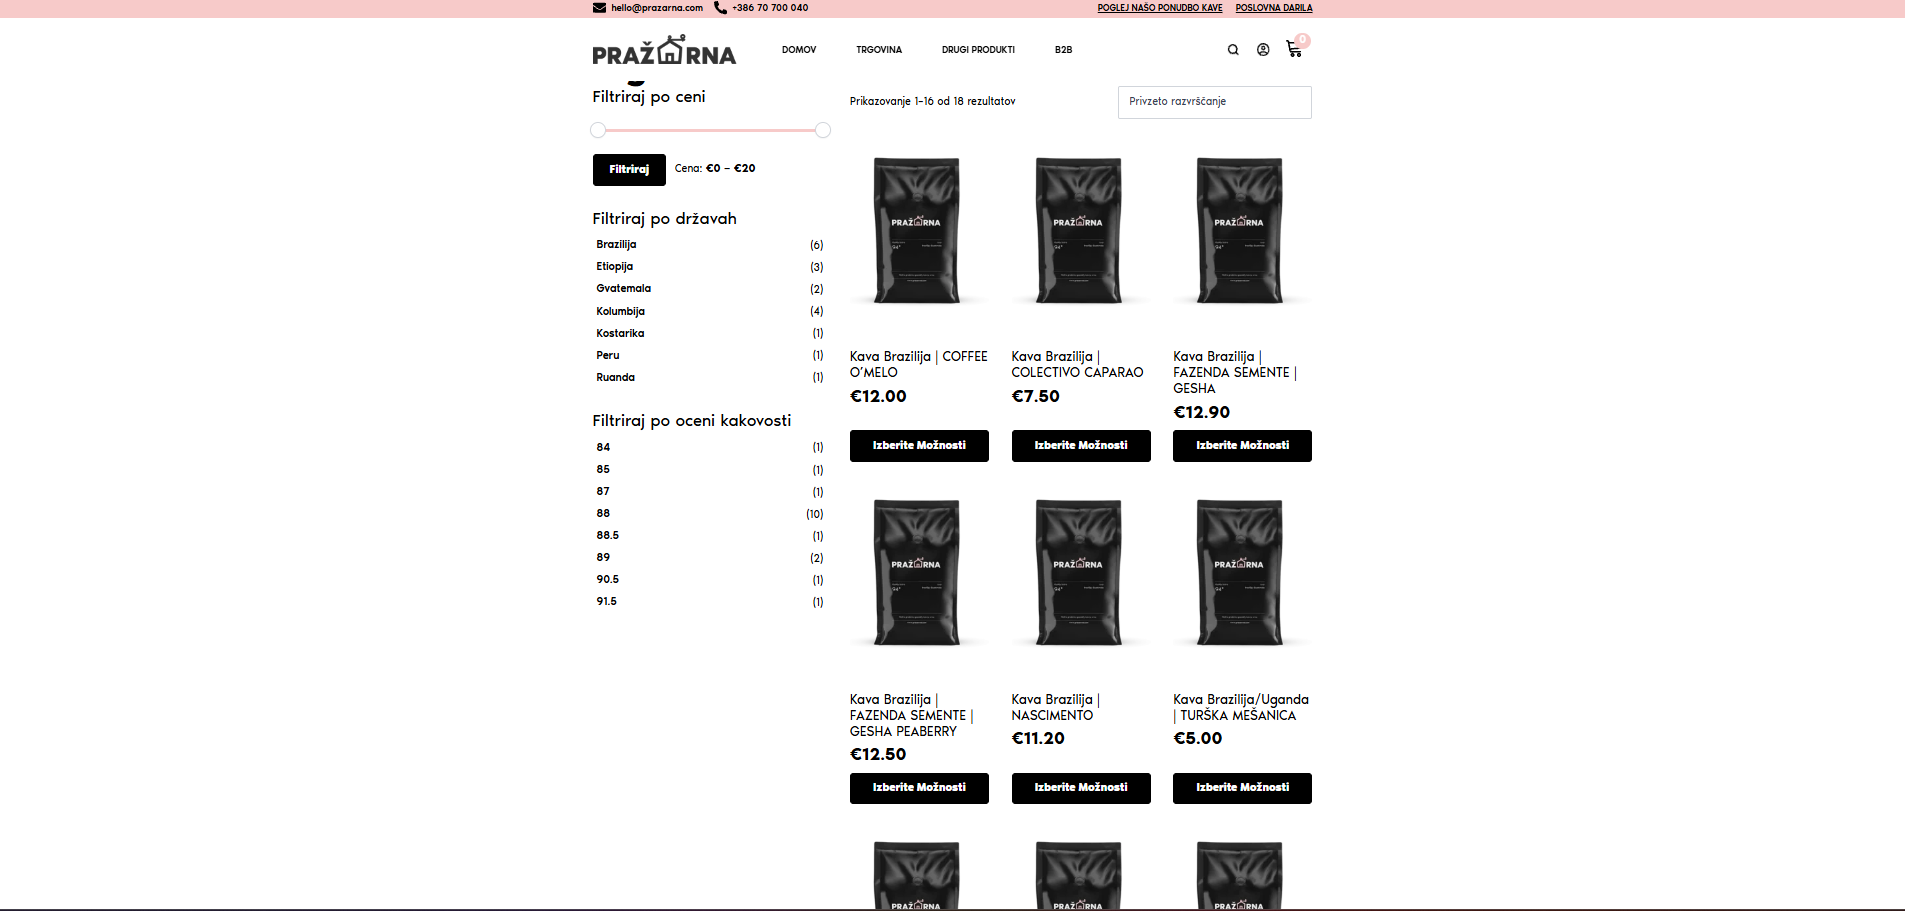
\includegraphics[width=1.0\textwidth]{slike/prazarna.png}
\caption{Posnetek zaslona spletne strani Pražarna \cite{prazarna}.}
\end{figure}
\newpage
\section{Zrno na zrno}
Zrno na zrno je spletna trgovina s kavo in pripomočki za njeno pripravo. V ponudbi so kavna zrna, mleta kava, kavni aparati in dodatki \cite{zrno}.

\textbf{Ključne funkcionalnosti:} filtriranje po ceni, znamki, zalogi, pakiranju in količini ter spletni nakup.

\textbf{Prednosti:} na enem mestu so različne vrste kave in oprema; kategorije kupcu pomagajo pri iskanju izdelkov.

\textbf{Slabosti (lastna ocena):} širok nabor opreme lahko preusmeri pozornost od same kave; za naš koncept je pomembnejša povezava med lokalno kavarno, praženjem in kupcem.
\begin{figure}[h!]
\centering
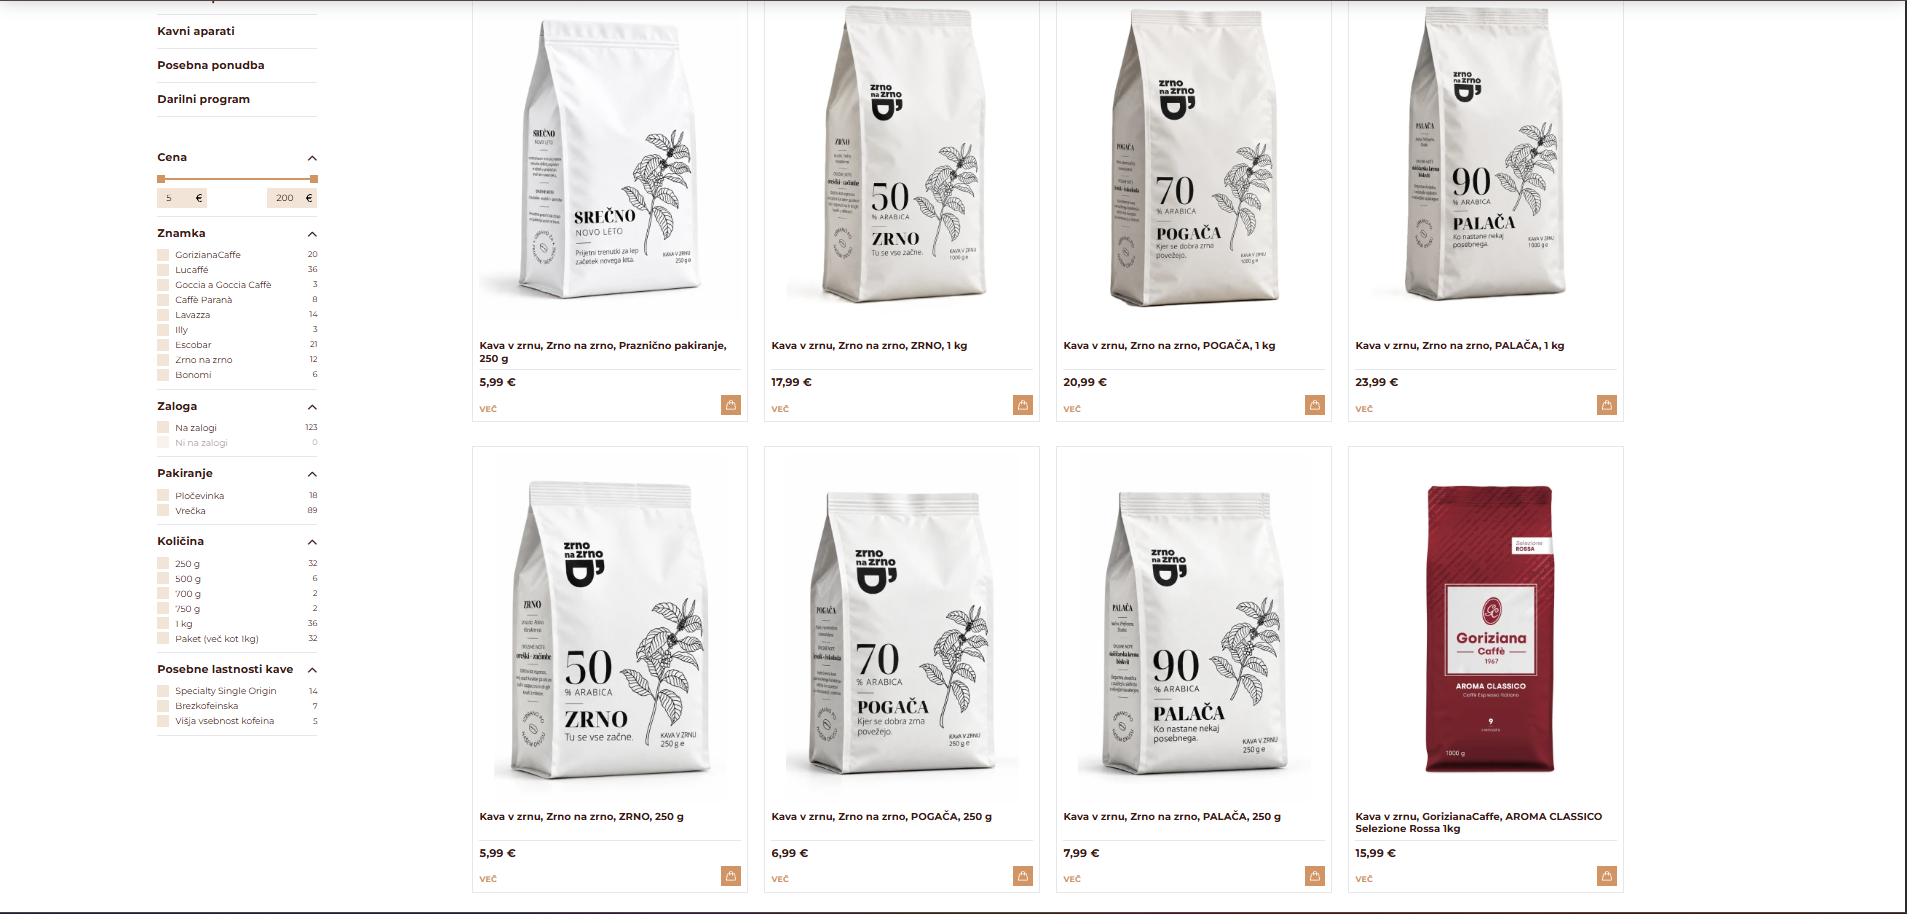
\includegraphics[width=1.0\textwidth]{slike/zrnonazrno.png}
\caption{Posnetek zaslona trgovine Zrno na zrno \cite{zrno}.}
\end{figure}
\newpage
\section{Zaključek}
Od Escobarja bomo prevzeli jasne opise porekla in okusov, od Pražarne izobraževalne vsebine in predstavitev poslovne ponudbe, od trgovine Zrno na zrno pa pregledno razvrščanje izdelkov.

Naša rešitev bo zasnovana tako, da bo kupcu olajšala izbiro kave tudi brez predhodnega znanja. Predvidene izboljšave so:
\begin{itemize}
\item preprost izbirnik kave glede na okus in način priprave;
\item jasni podatki o poreklu in datumu praženja;
\item možnost spletnega naročila in predvidenega osebnega prevzema v kavarni;
\item predstavitev lokalne skupnosti, trajnostne embalaže in dogodkov;
\item ločena ponudba za posameznike in podjetja.
\end{itemize}
Cilj je povezati spletni nakup s prijetno izkušnjo v fizični kavarni. Navedene izboljšave so predlogi za razvoj in ne trditve, da jih konkurenti nimajo.
\begin{thebibliography}{9}
\bibitem{escobar} Escobar. \emph{Kava -- spletna trgovina}. \url{https://escobar.si/slo/nasa-ponudba/kava.html}. Dostop: 24. 11. 2026.
\bibitem{prazarna} Pražarna. \emph{Uradna spletna stran}. \url{https://prazarna.com/}. Dostop: 24. 11. 2026.
\bibitem{zrno} Zrno na zrno. \emph{Spletna trgovina}. \url{https://zrnonazrno.si/}. Dostop: 24. 11. 2026.
\end{thebibliography}
\end{document}
